\documentclass{scrartcl}

\usepackage[utf8]{inputenc}
\usepackage[T1]{fontenc}
\usepackage{lmodern}
\usepackage[english]{babel}
\usepackage{amsmath}
\usepackage{graphicx}
\usepackage{caption}	
\usepackage{subcaption}	 
\usepackage{hyperref}
\usepackage[parfill]{parskip}
\usepackage{hhline}
\usepackage{subcaption}

\title{Neuroprosthetics - Exercise 8}
\author{Alexander Koenig}
\date{31. January 2019}

\begin{document}
\maketitle

\section{Noise Vocoder with Dynamic Compression}

In this exercise, a noise vocoder with dynamic compression is implemented to model the sound impressions a patient using a cochlear implant (CI) is hearing. In order for this to work white noise with a Gaussian distribution (mean 0, standard deviation 1) is filtered with the filter banks from exercise 7. The filtered noise is then modulated with the envelopes of a filtered speech signal. The envelopes are generated with a Hilbert transform. The envelopes for a CI with 12 electrodes are displayed in figure \ref{fig:envelopes}. The same word ("Koenigs Test Word") as in the previous exercise is used in this exercise. 

\begin{figure}[h]
	\vspace{0.5cm}
	\centering
	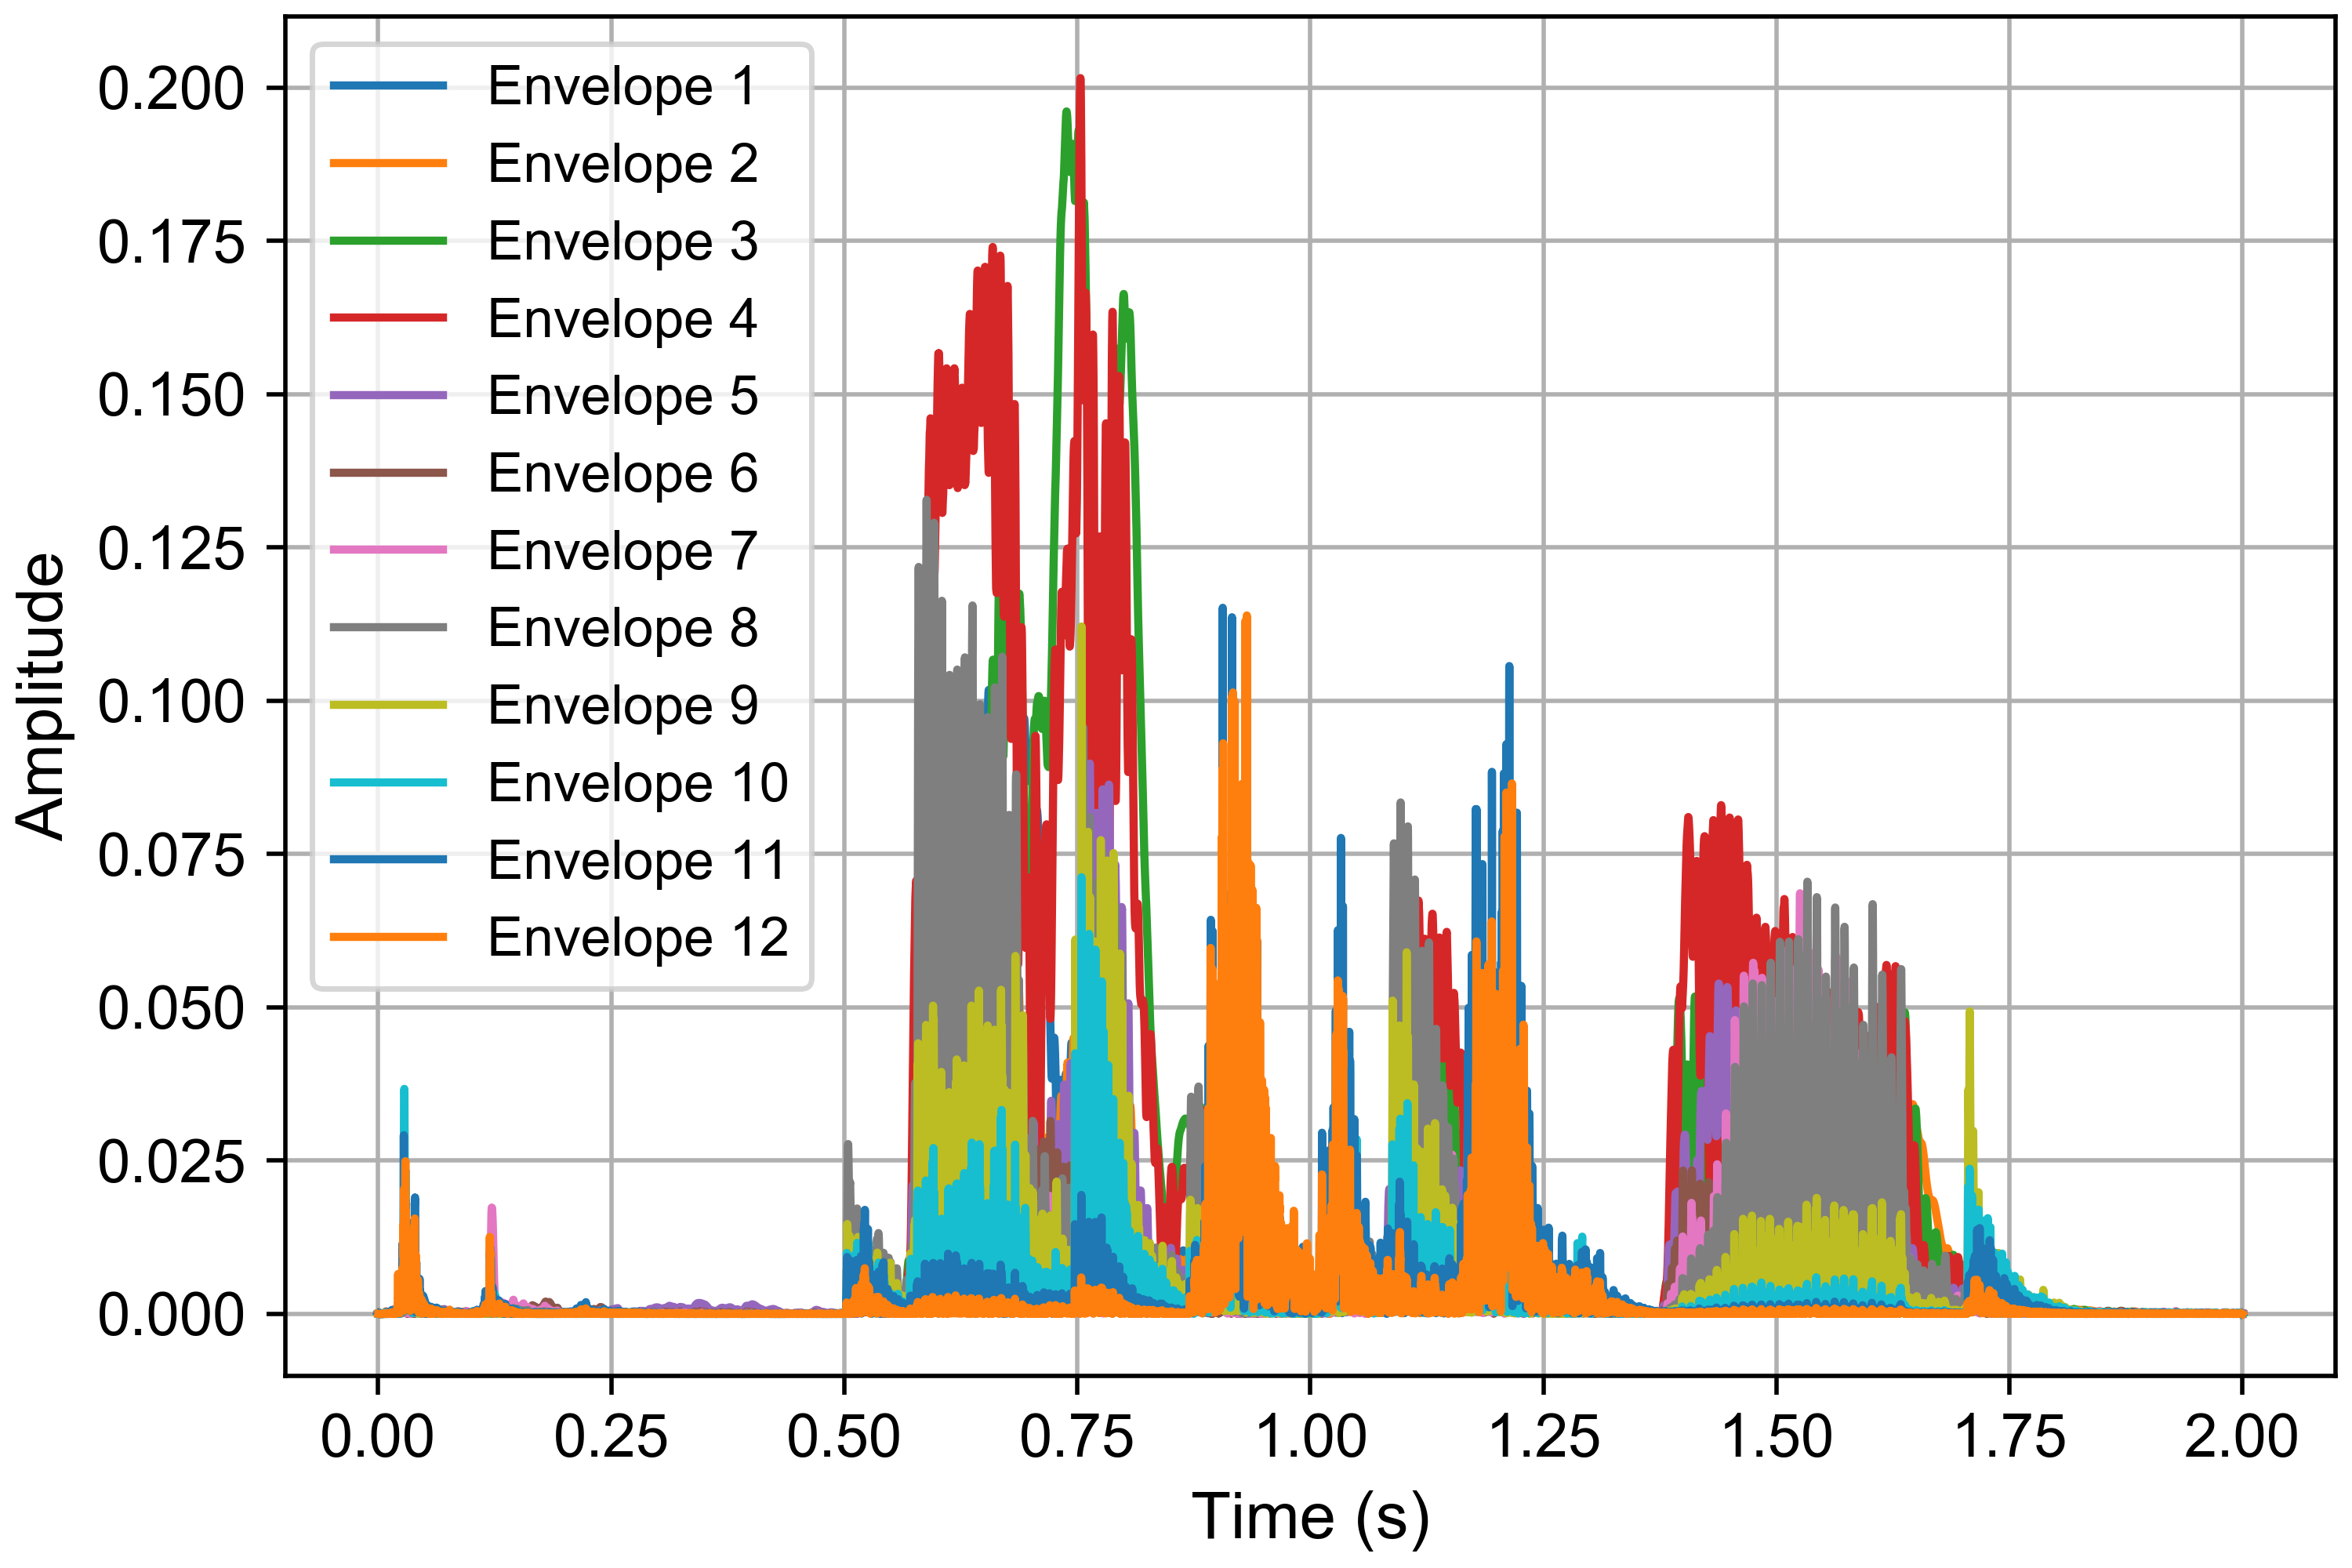
\includegraphics[width=0.9\textwidth]{figures/envelopes}
	\caption{Envelopes for 12 electrode-CI}
	\label{fig:envelopes}
\end{figure}

\newpage
In the next step dynamic compression according to equation 1 is applied to the envelopes. The variable $c$ is the compression rate, which is set to 500. After the compression, all values above a threshold of 1 are clipped to a value of 1 and all values below a custom threshold are clipped to 0. Figure \ref{fig:proc_envelopes} shows the processed envelopes with a lower threshold of 0.2. It is obvious that the higher threshold of 1 is never reached, but all amplitudes below 0.2 are clipped to 0.

\begin{equation}
\mathrm{env_{compressed}}=\frac{\log _{10}(1+c \cdot \mathrm{env})}{\log _{10}(c+1)}
\end{equation}

\begin{figure}[h]
	\vspace{0.5cm}
	\centering
	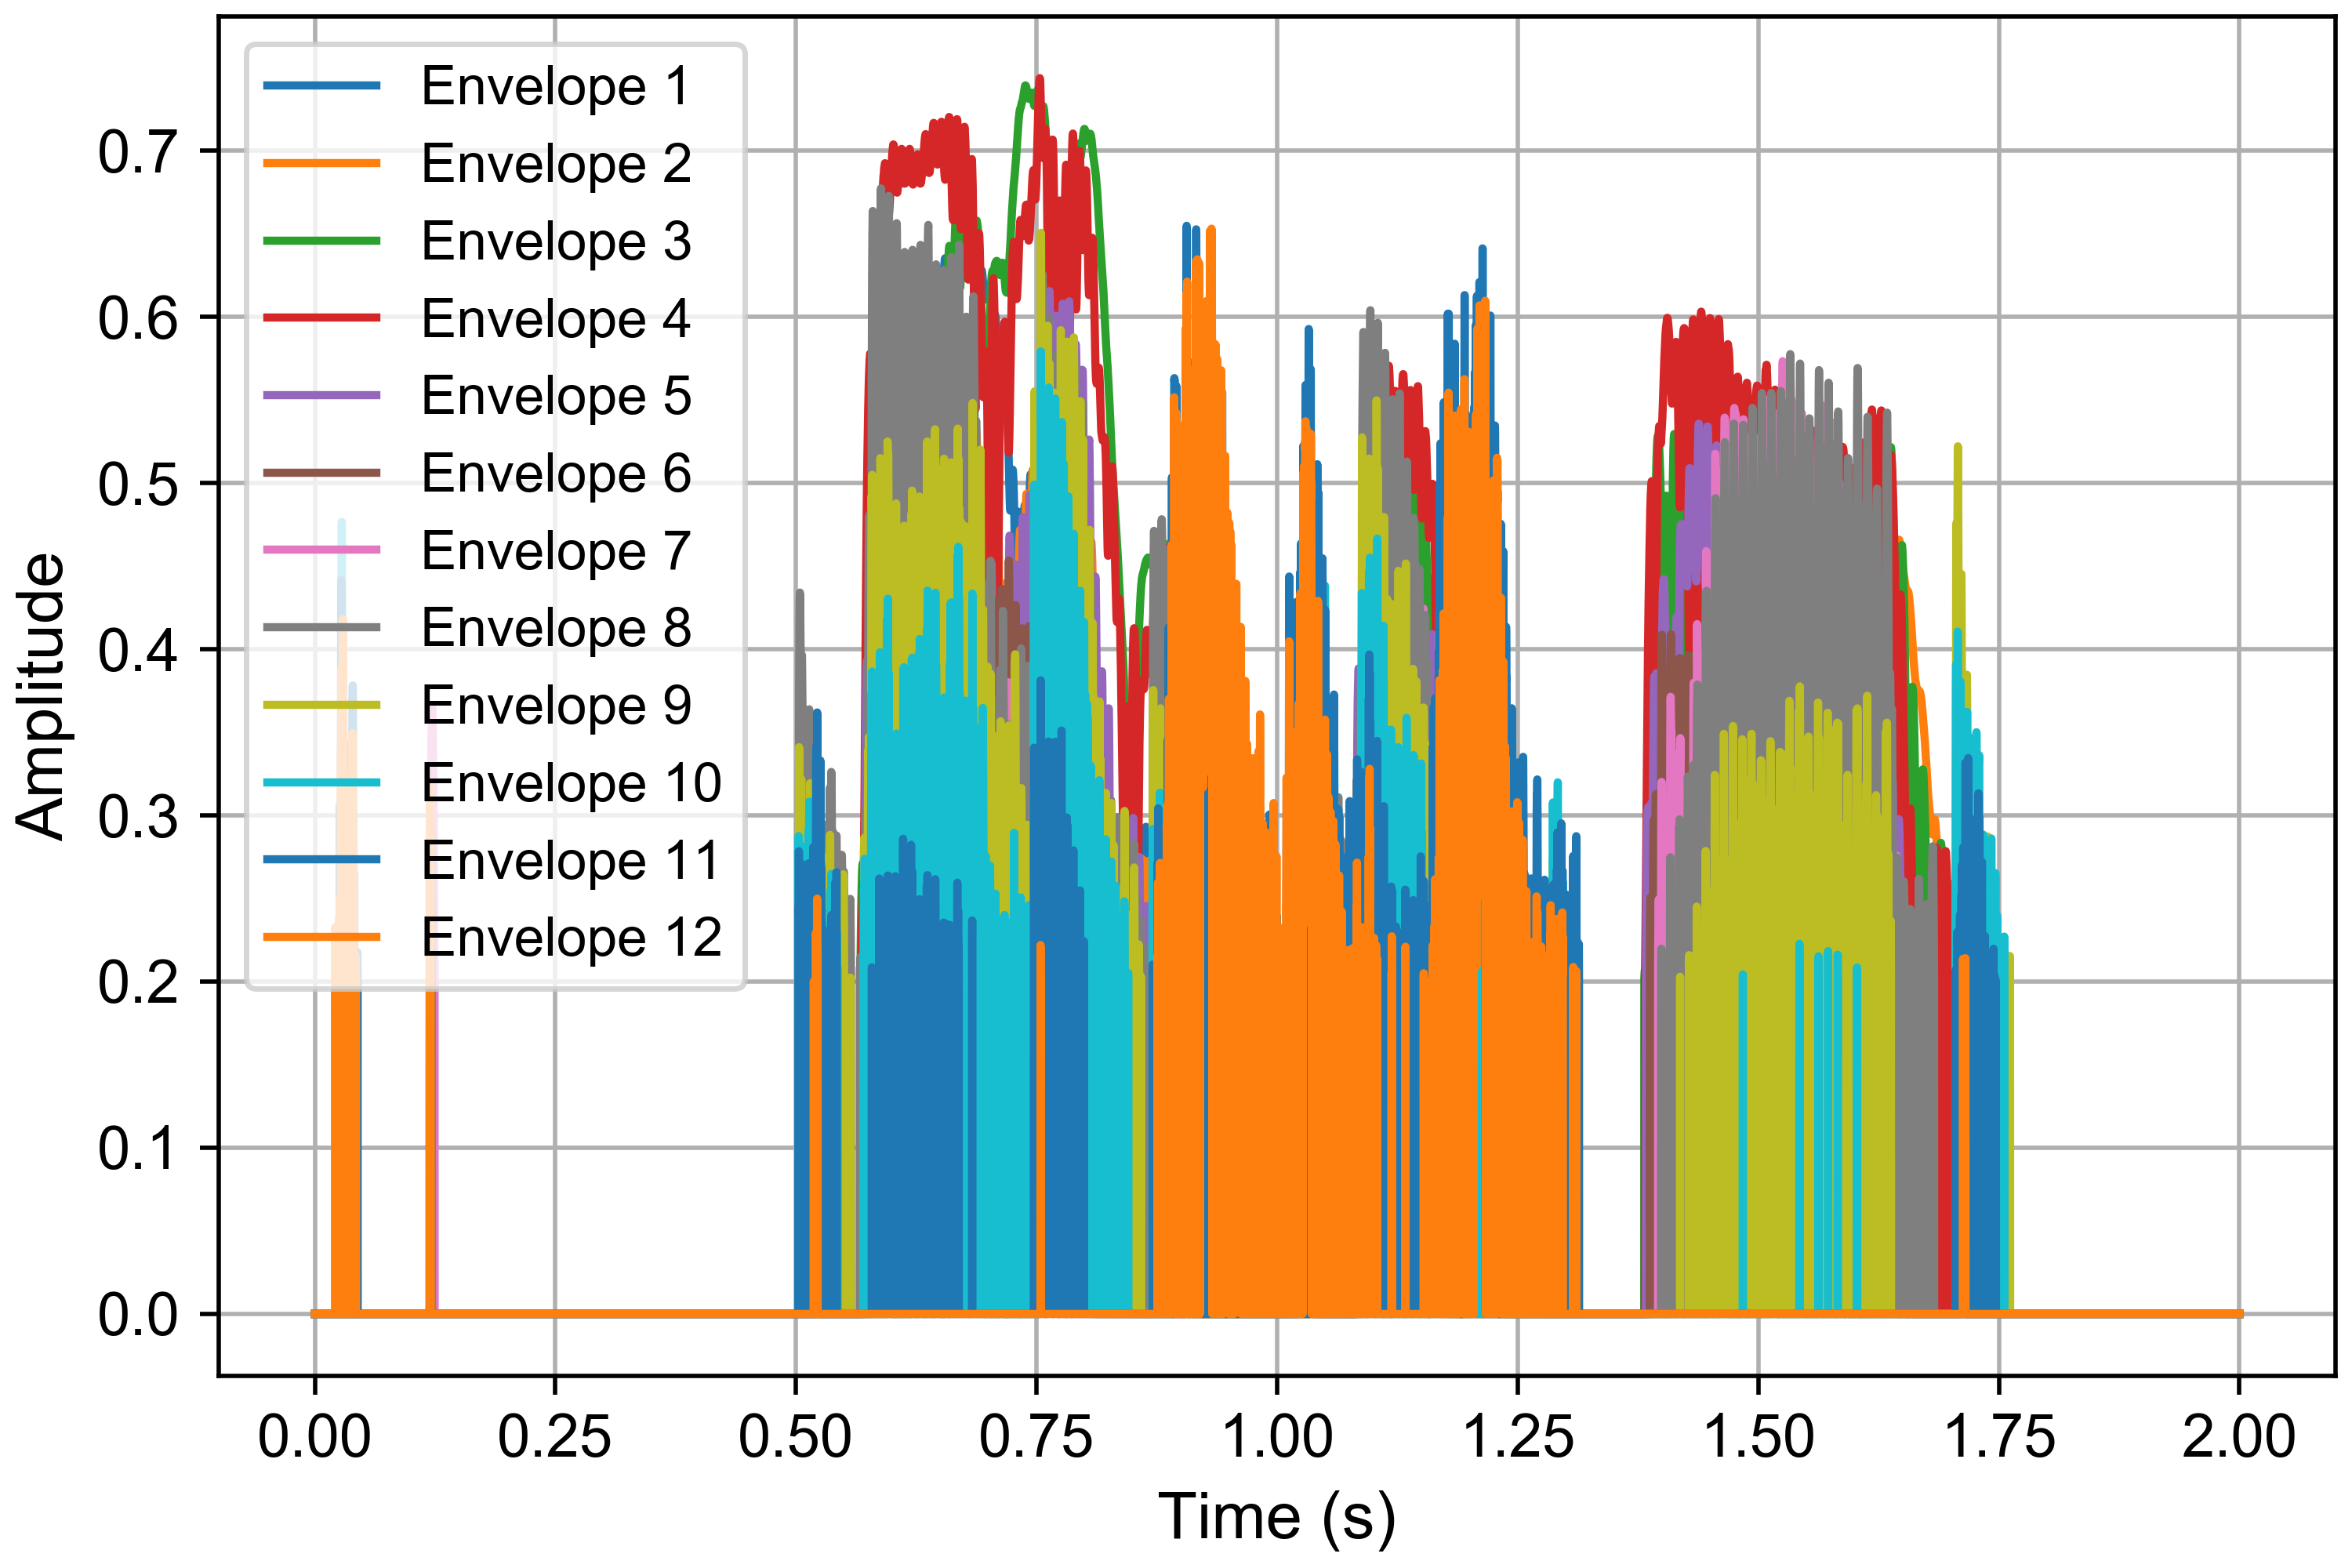
\includegraphics[width=0.9\textwidth]{figures/proc_envelopes}
	\caption{Compressed and filtered envelopes for 12 electrode-CI}
	\label{fig:proc_envelopes}
\end{figure}

\vspace{0.5cm}
In the next step, the processed envelopes are modulated with the noise to model the signal that the patient will hear. After this, the signals at each electrode of the CI are summed back together to get an overall acoustic impression. Figures \ref{fig:amp}, \ref{fig:spectrum} and \ref{fig:spectrogram} show the amplitudes, the spectra and the spectrograms of the original and the reconstructed signal for a 12-electrode CI, respectively.

Figure \ref{fig:amp} demonstrates that the reconstruction process with the introduced noise "smudges" out the signal. The peaks are less distinct, making the signal less intelligible. Also, the amplitude of the signal is increased. Figure \ref{fig:spectrum} shows that the induced noise is also visible in the power spectrum. Almost all frequencies have a power greater than zero - which comes from the white noise generated in the beginning. Finally, figure \ref{fig:spectrogram} shows that the words (three dark red areas in the top figure) are less distinct in the noisy reconstruction. Further, some parts of the signal do not appear in the spectrogram at all because the amplitude of the compressed envelope was below the clipping threshold.

When listening to the summed up signals, which represent the signal the patient hears, it becomes clear that the more electrodes the CI has, the better the reconstruction quality becomes. While the signal for 3 electrodes is almost not understandable and purely noise, the word reconstructed by a 22-electrode CI can be understood well. Increasing the threshold from 0.2 to higher values removes more parts of the signal and hence reduces the comprehensibility of the word. At lower compression rates the signal seemed to be better intelligible than for higher ones. Higher-order (e.g. order 8) bandpass filters only produced loud noises and no good reconstruction. Using lower order (e.g. order 2) filters seems to produce lower quality results. 

\begin{figure}[p]
	\centering
	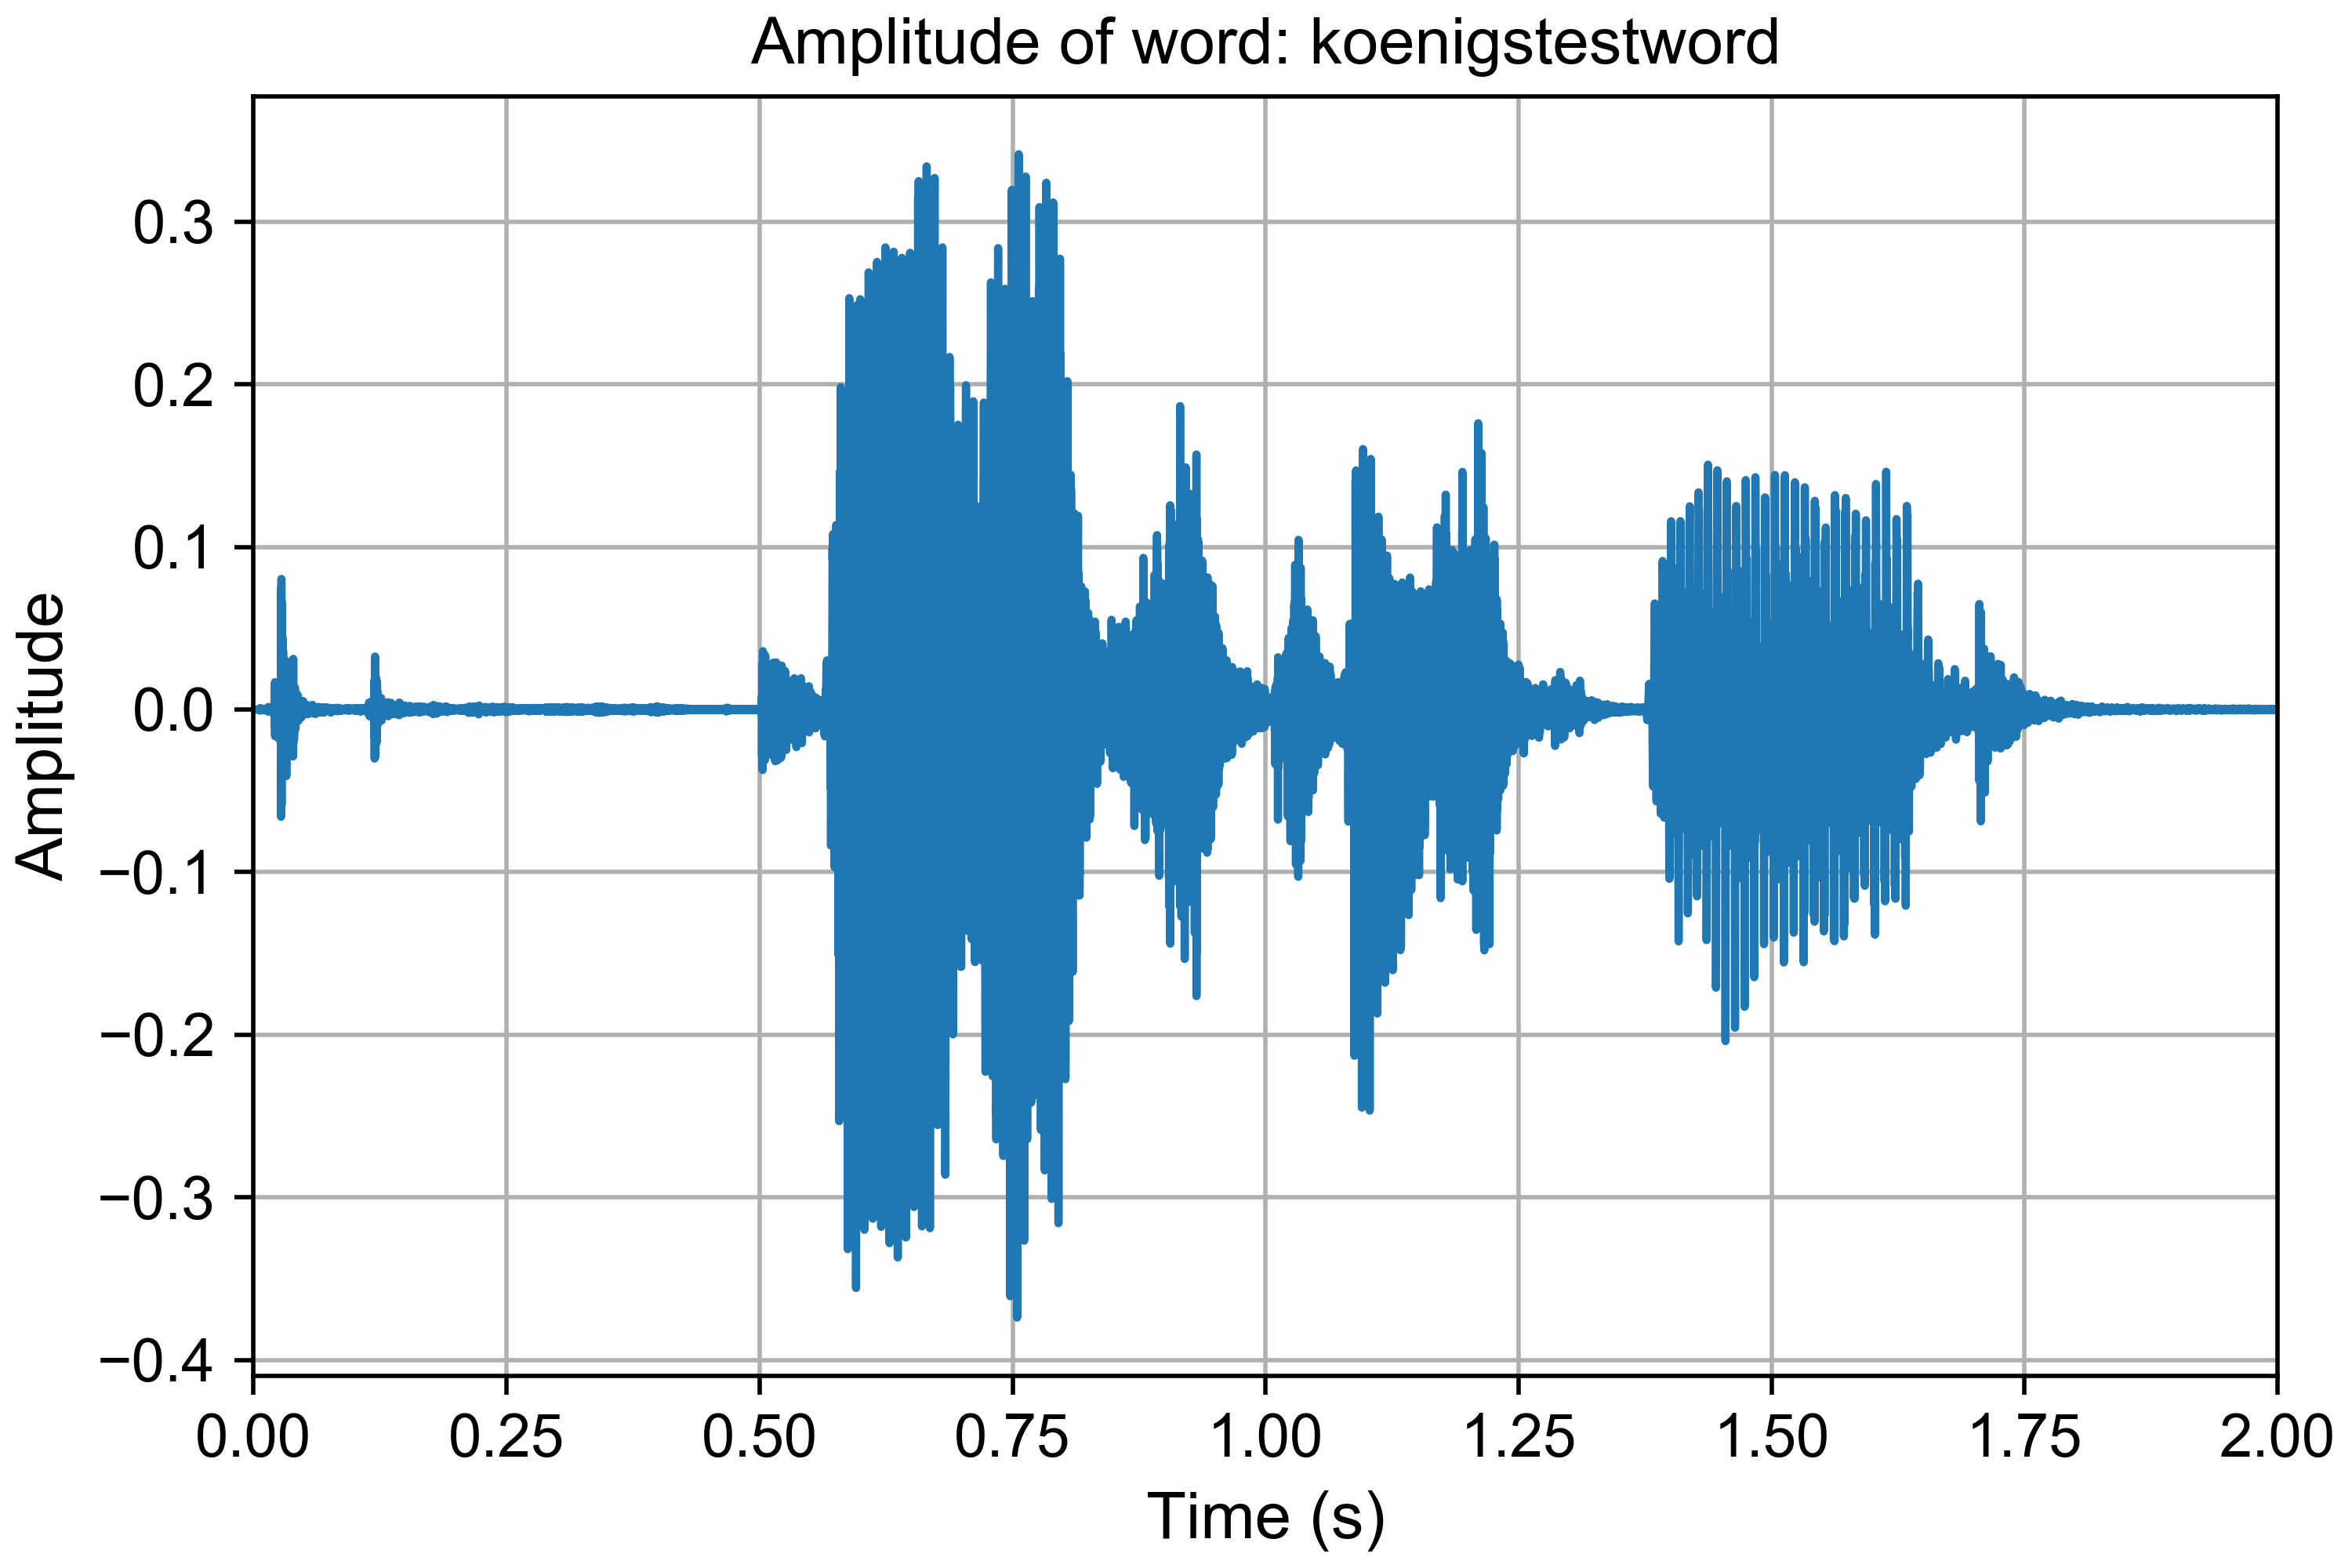
\includegraphics[width=0.9\textwidth]{figures/amplitude_koenigstestword}
	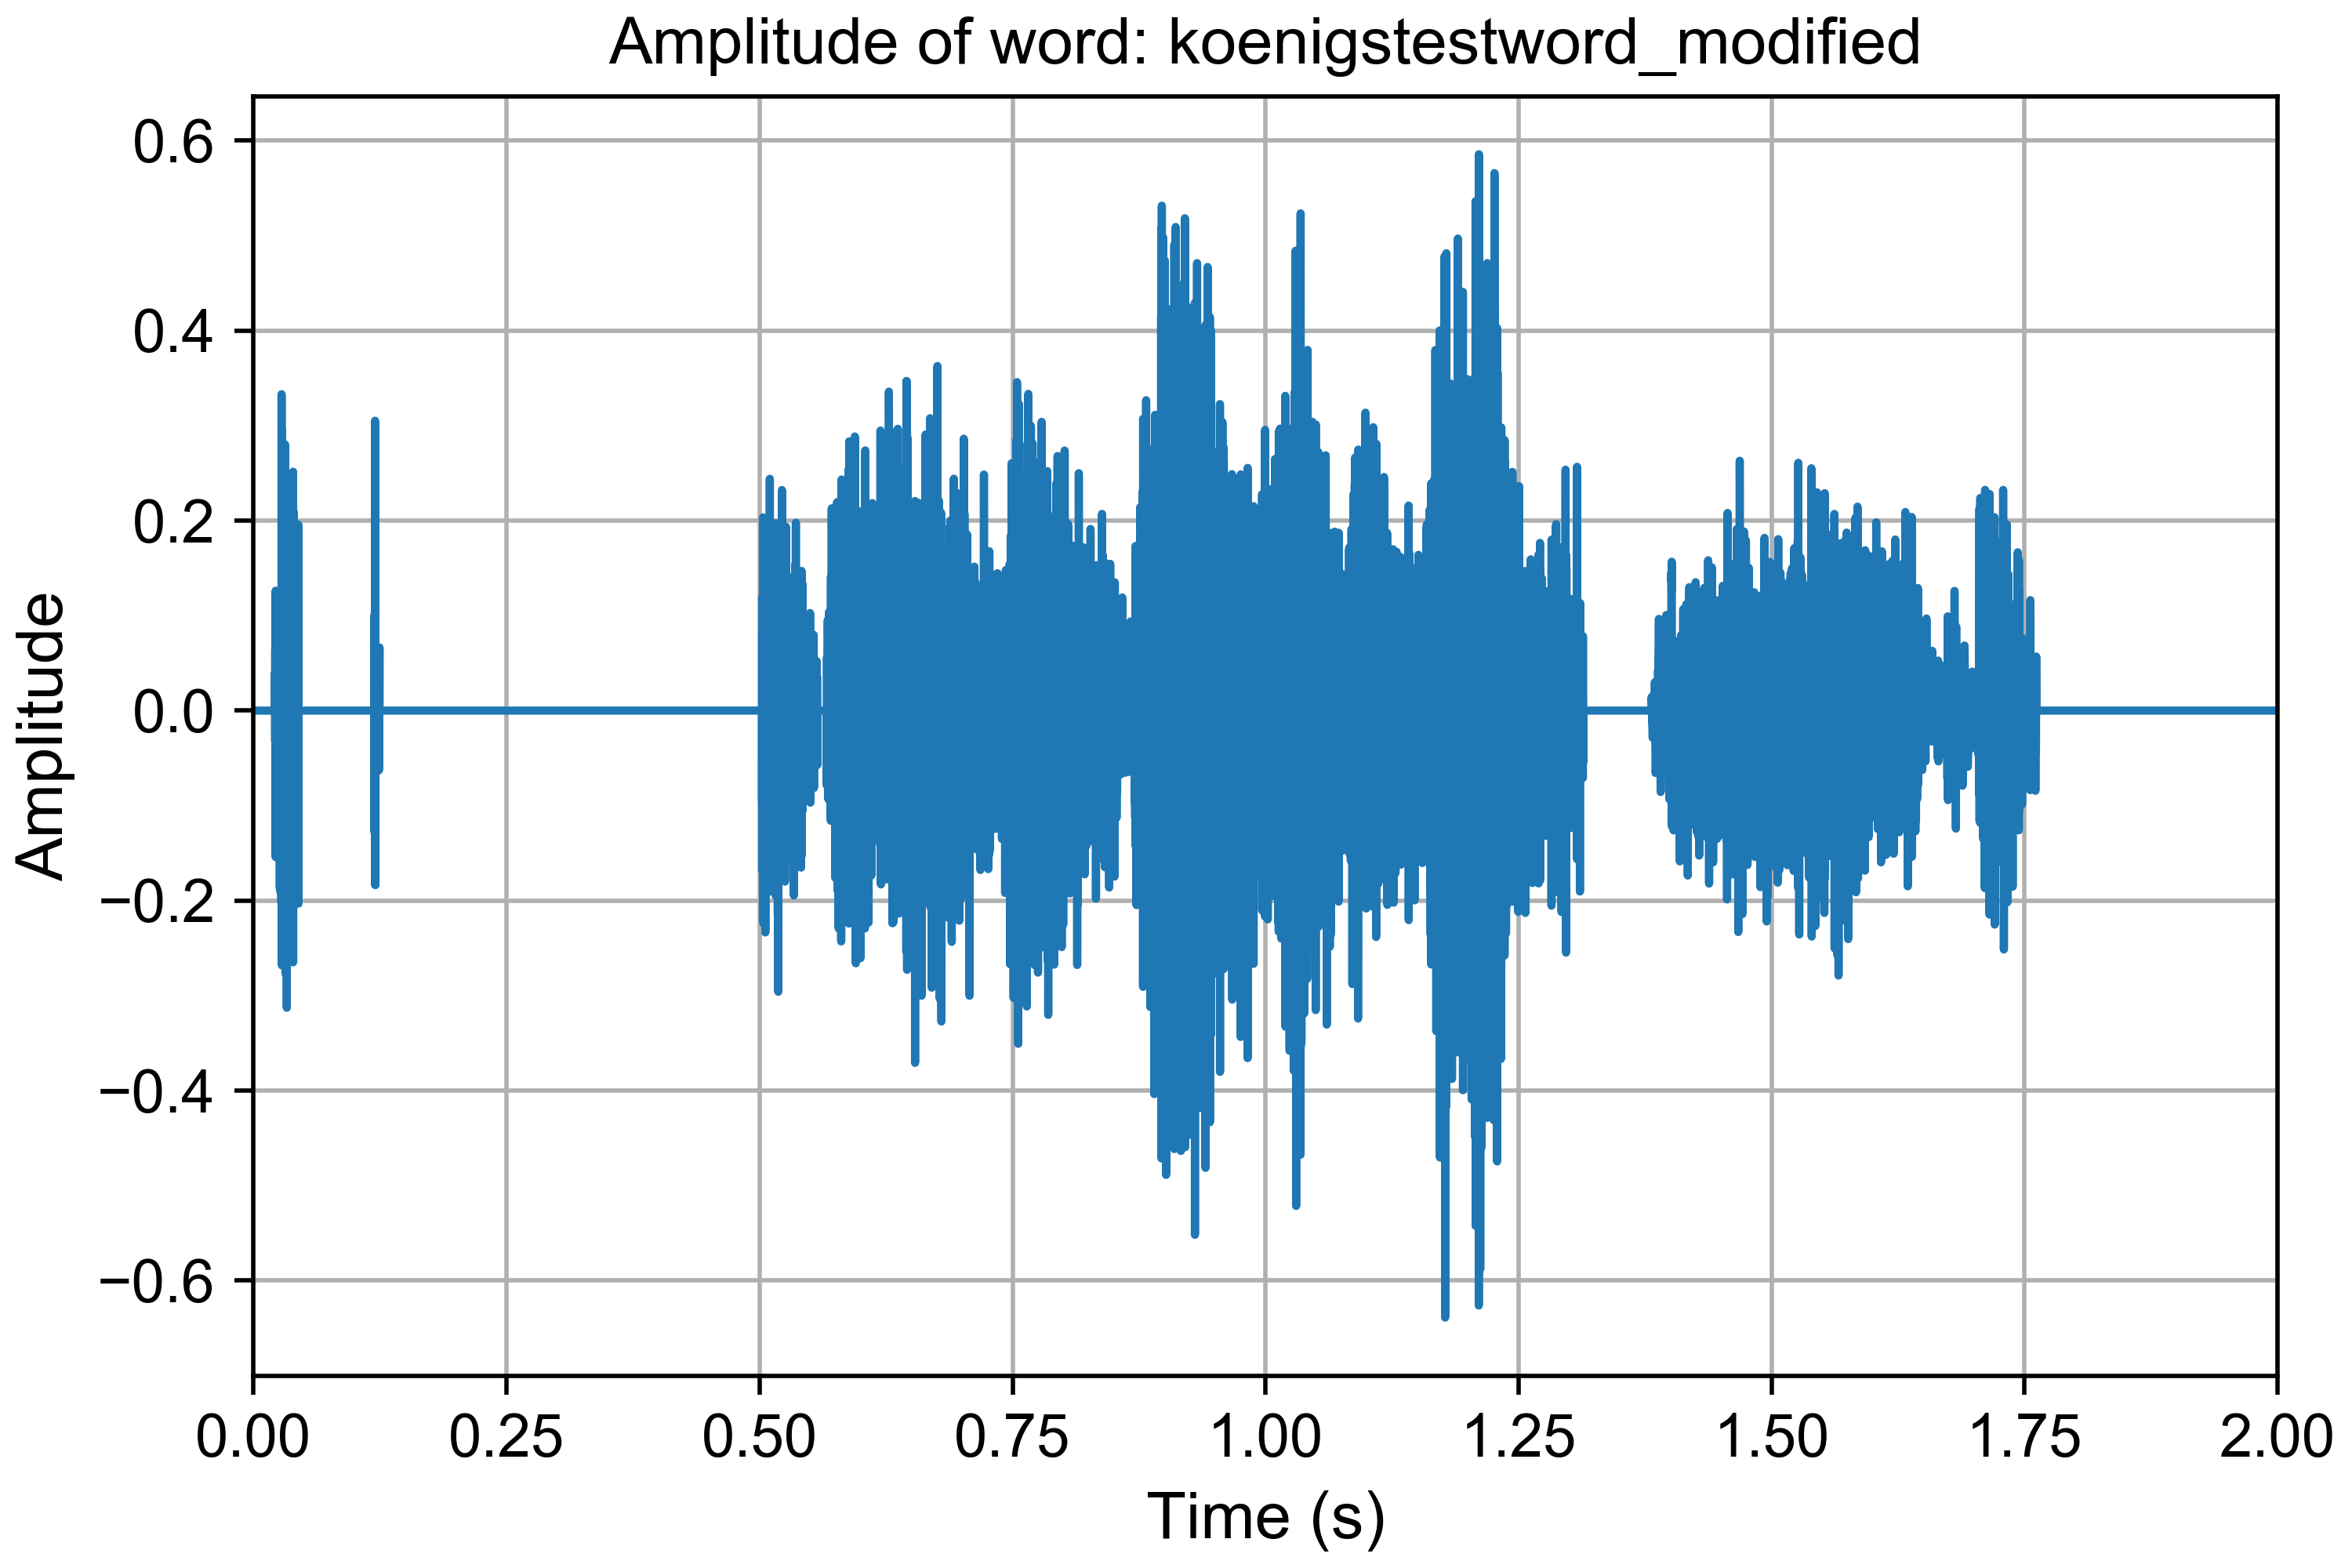
\includegraphics[width=0.9\textwidth]{figures/amplitude_koenigstestword_modified}
	\caption{Amplitudes of original and reconstructed signals}
	\label{fig:amp}
\end{figure}

\begin{figure}[p]
	\centering
	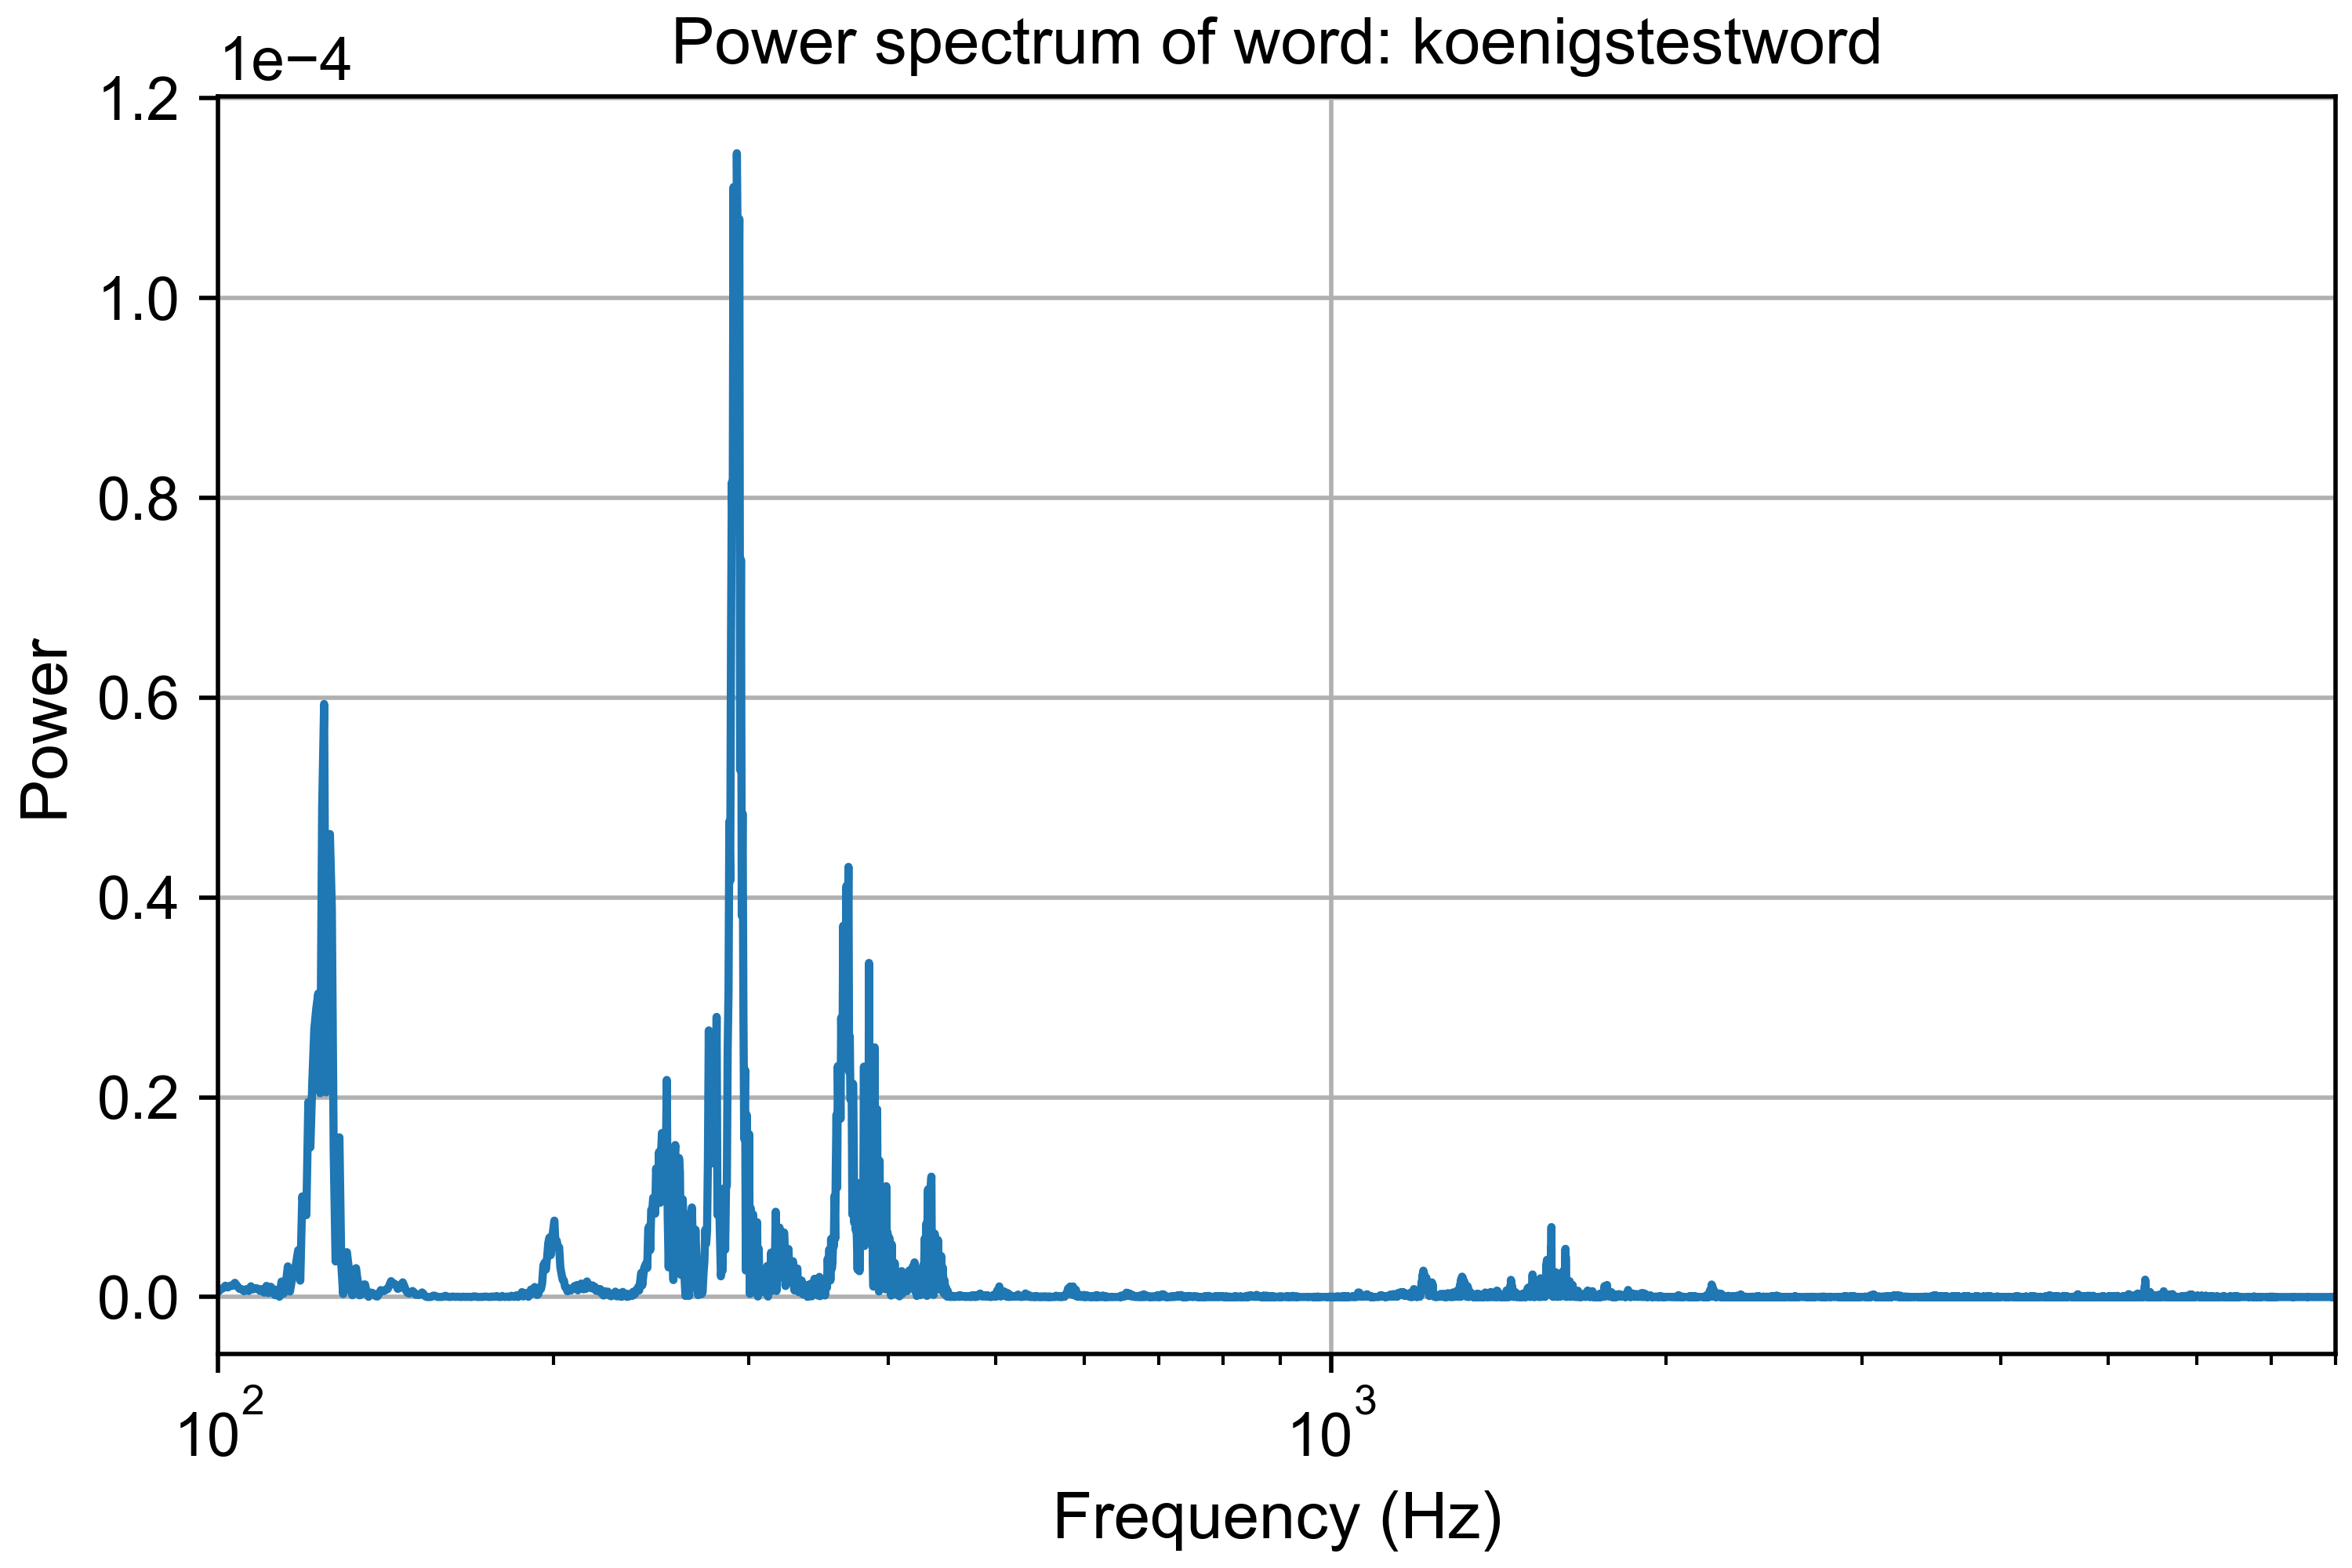
\includegraphics[width=0.9\textwidth]{figures/spectrum_koenigstestword}
	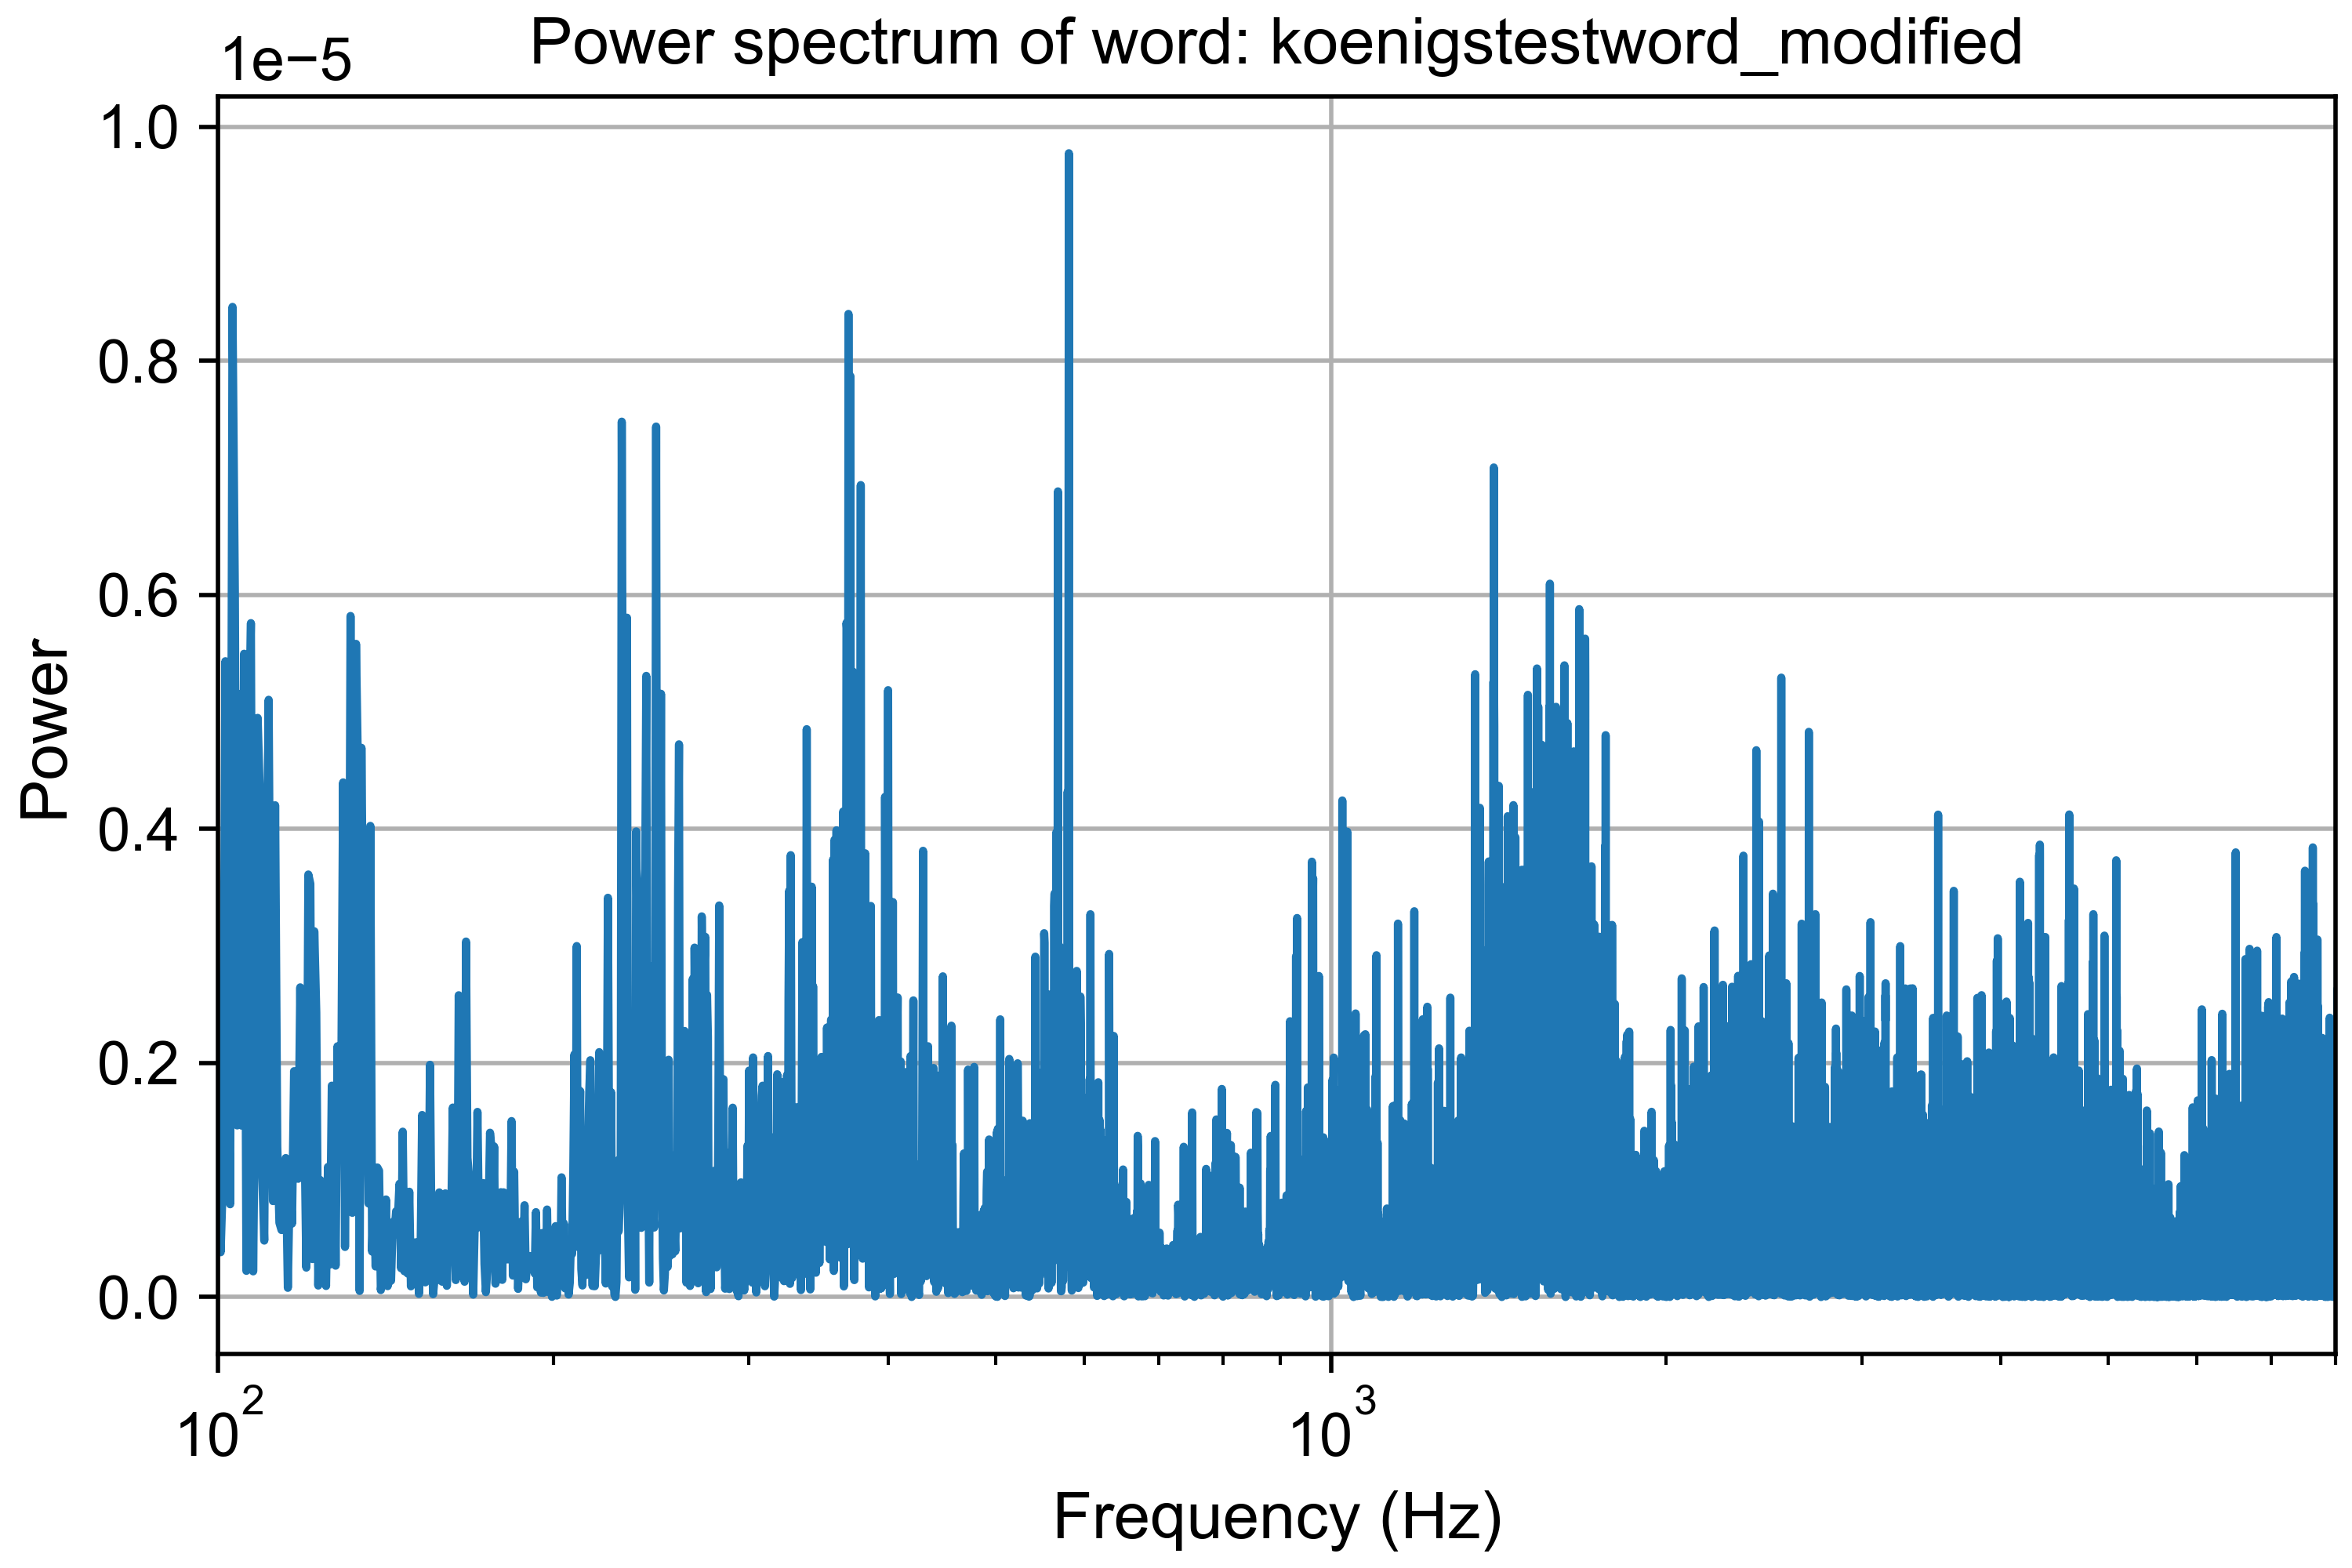
\includegraphics[width=0.9\textwidth]{figures/spectrum_koenigstestword_modified}
	\caption{Spectra of original and reconstructed signals}
	\label{fig:spectrum}
\end{figure}

\begin{figure}[p]
	\centering
	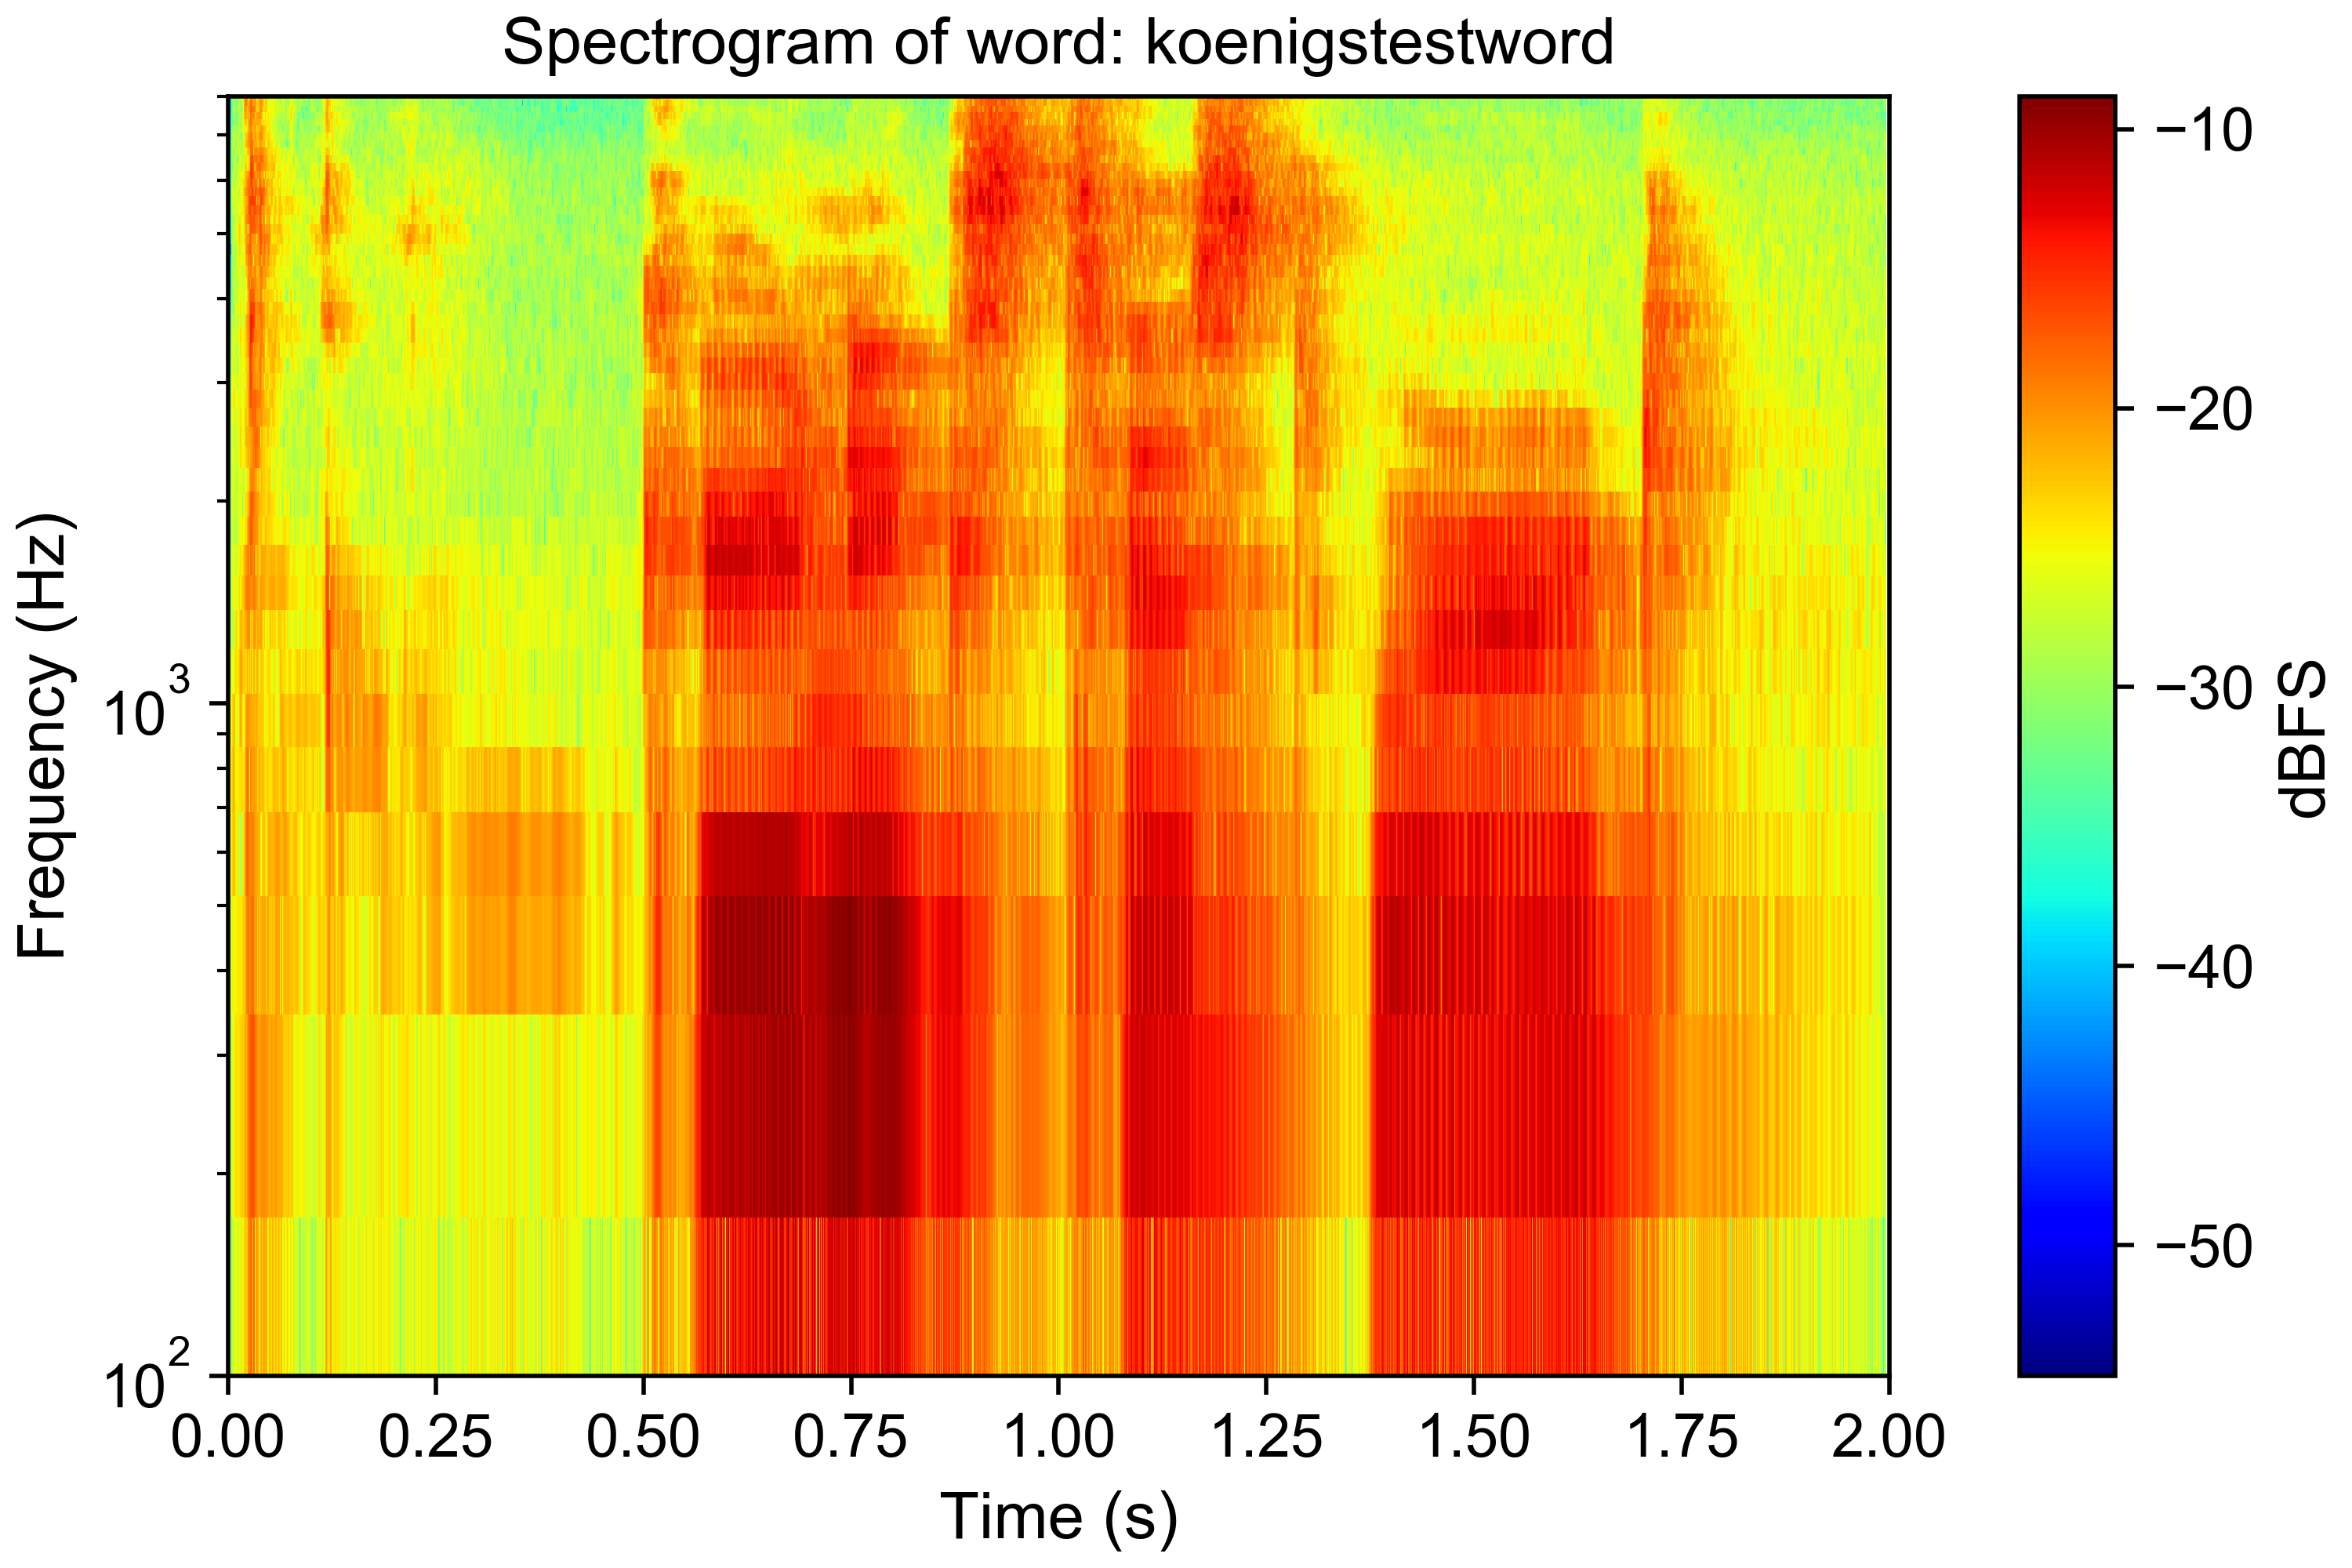
\includegraphics[width=0.9\textwidth]{figures/spectrogram_koenigstestword}
	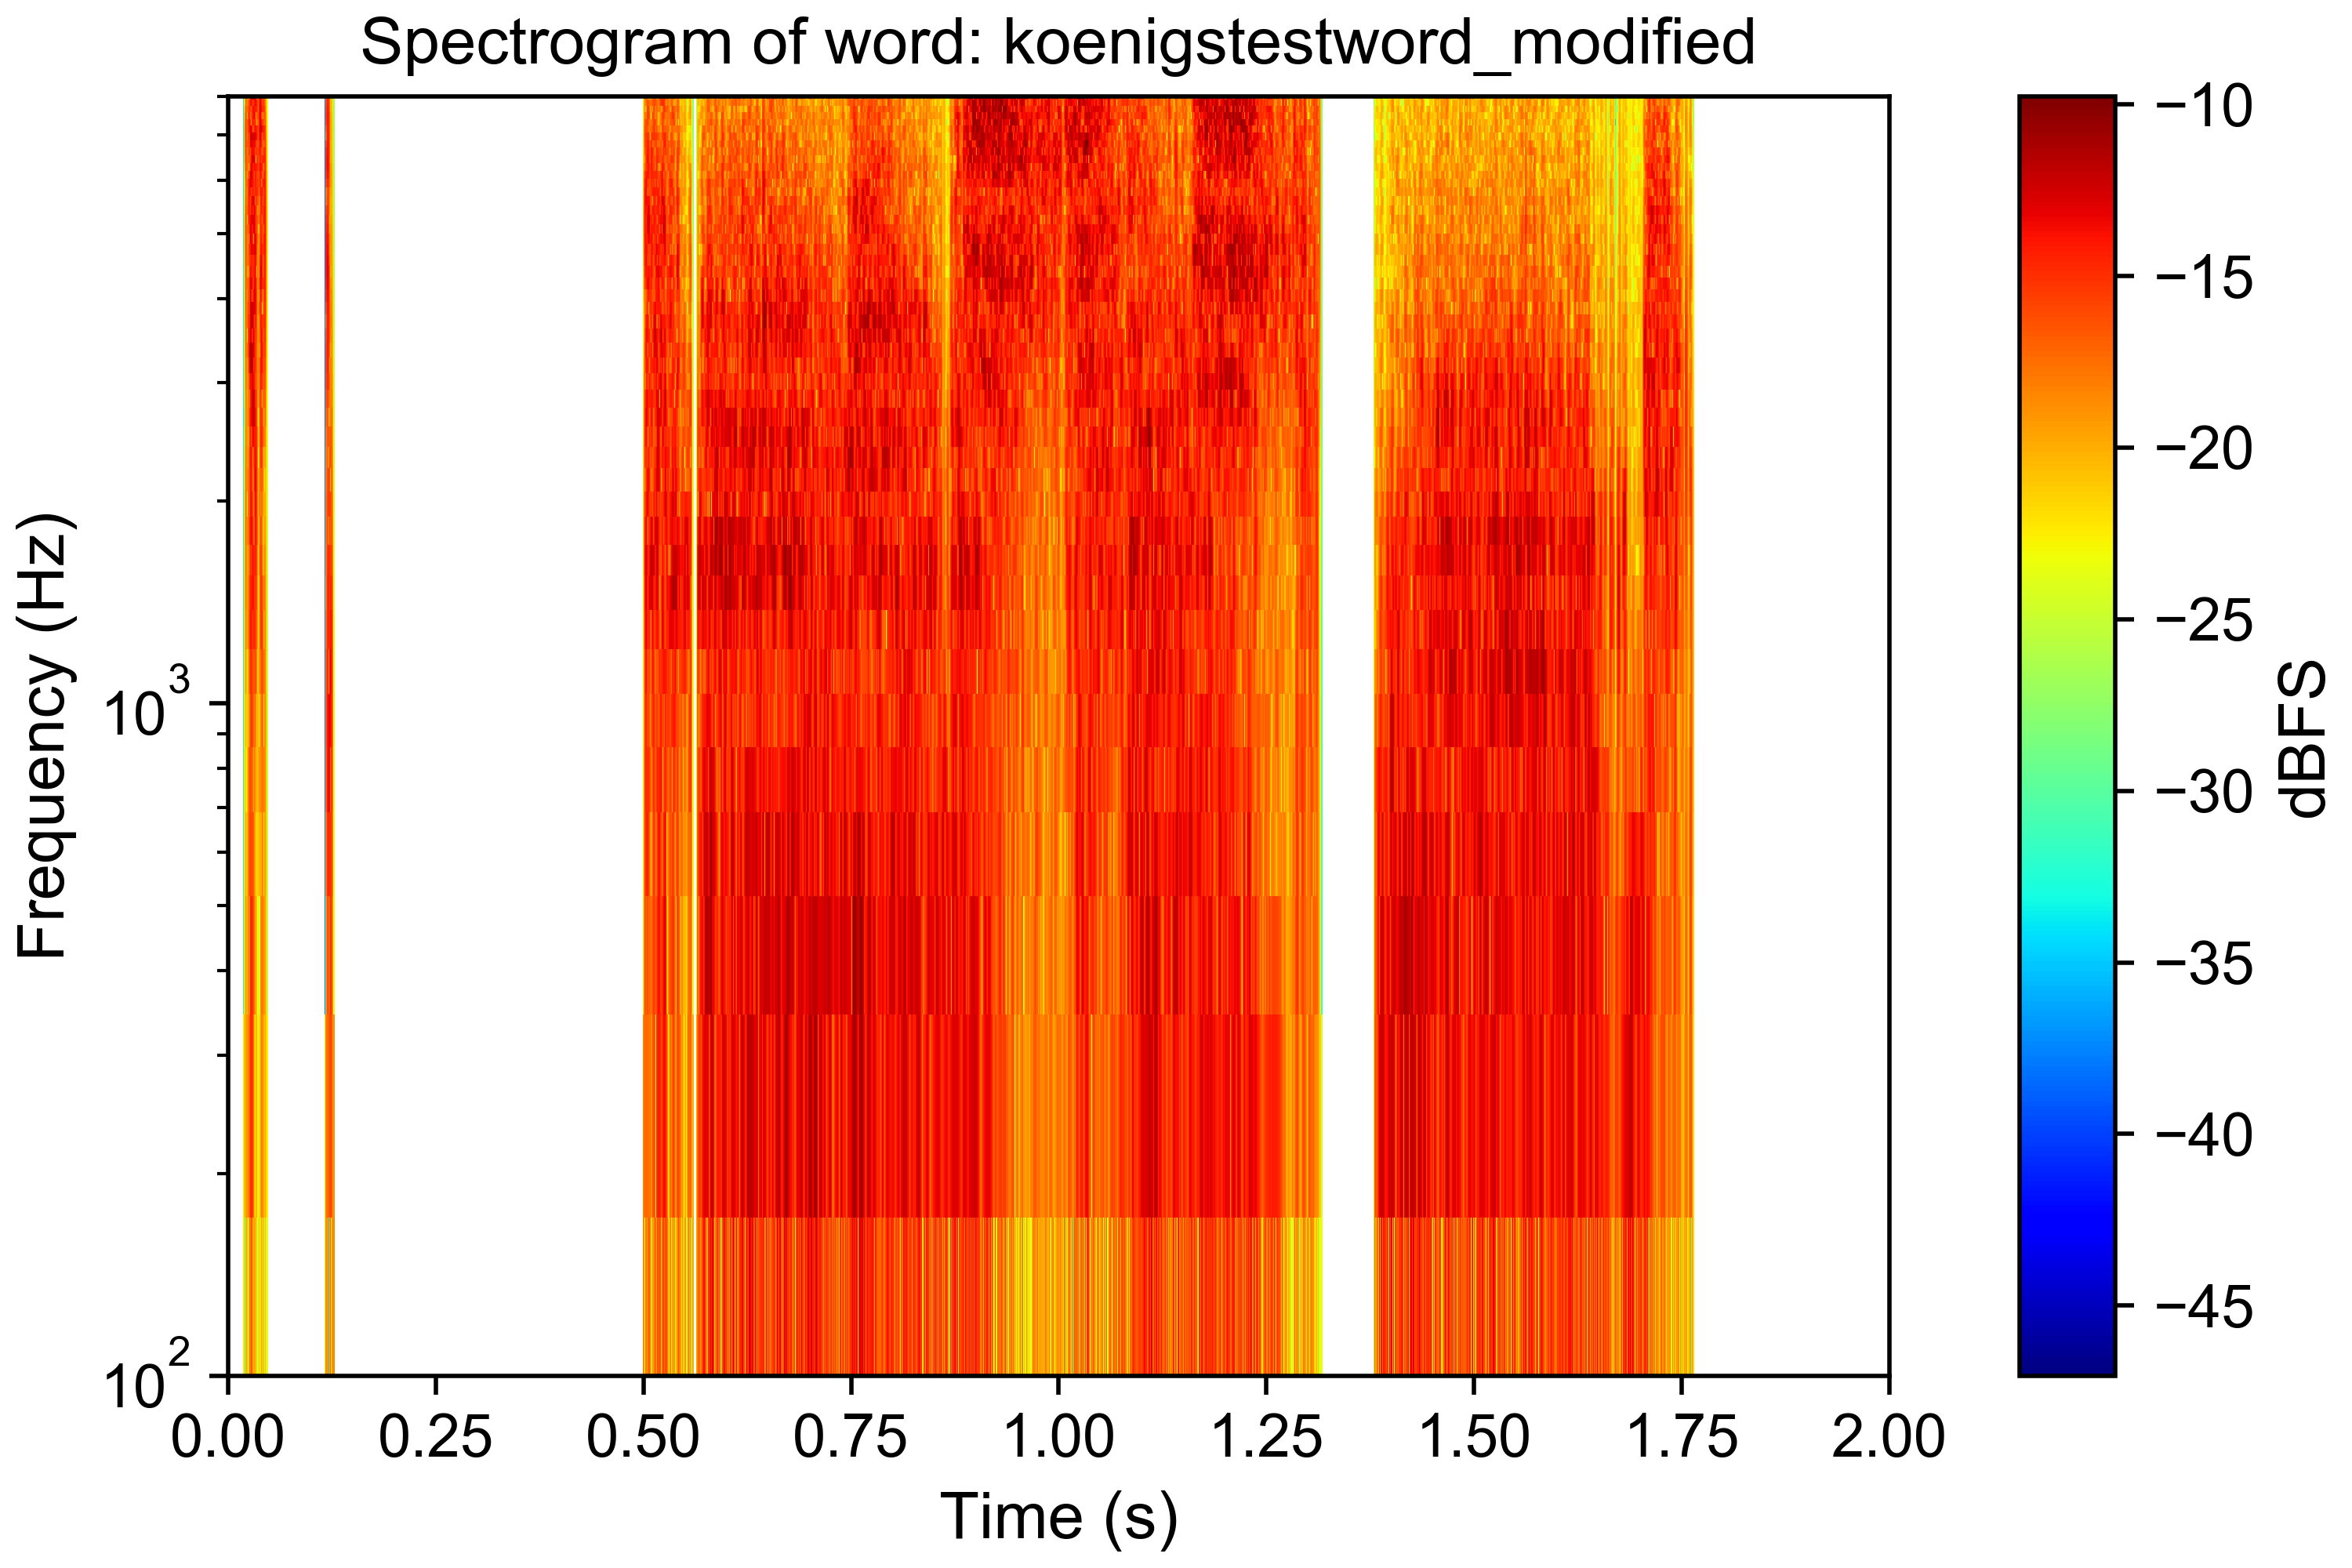
\includegraphics[width=0.9\textwidth]{figures/spectrogram_koenigstestword_modified}
	\caption{Spectrograms of original and reconstructed signals}
	\label{fig:spectrogram}
\end{figure}

\end{document}